Eine Kraft gibt an, wie stark ein Körper mit einer definierten Masse beschleunigt wird, wenn diese Kraft auf ihn einwirkt. 


\subsection{Sichtbarkeit}

Kräfte sind unsichtbar. Man kann allein deren Auswirkung, beispielsweise das Beschleunigen eines Körpers oder Verformung beobachten und auf eine Kraftwirkung schließen.


\subsection{Einheit}

Kräfte haben die Einheit $N$ (sprich: \glqq Newton\grqq ), welche, ausgeschrieben in SI-Basiseinheiten, $\frac{kg \cdot m}{s^2}$ entspricht. Dies lässt sich aus Newtons 2. Axiom ableiten:

Da die Basiseinheit für Masse $kg$ und die Einheit für Beschleunigung $\frac{m}{s^2}$ ist (Geschwindigkeit pro Zeit: Meter pro Sekunde pro Sekunde: $\frac{\frac{m}{s}}{s}=\frac{m}{s^2}$), folgt die Definition des Newtons direkt aus $F = m \cdot a$.


\subsection{Richtung}

Da Kräfte gerichtete Größen sind, geben sie nicht nur den Betrag der Kraft sondern auch eine Richtung an, in welche sie auf einen Körper wirken, weshalb sie in Formeln oft als Vektor $\vec{F}$ geschrieben werden, um diese Eigenschaft anzuzeigen.

\begin{Anmerkung}
In der Schulphysik ist es allerdings nur wichtig, diese Eigenschaft zu kennen, um Kräfteparallelogramme zu begründen, Vektorrechnungen werden nicht vollzogen. Sollte die Richtung einer Kraft für eine Aufgabe von Bedeutung sein, wird mit Winkelbeziehungen hergeleitet.
\end{Anmerkung}

\subsection{Kräfteaddition} \label{subsec:kraefteaddition}

Wenn mehrere Kräfte auf einen Körper wirken, dann gibt es eine resultierende Kraft ($F_{res}$ oder $F_{ges}$ geschrieben), welche die Addition der beiden ist. Diese Addition muss aber grafisch vollzogen werden, da nicht nur die Beträge, sondern auch deren Richtungen zählen; zwei gleich große Kräfte, die einander entgegengesetzt sind, sind in der Addition $0$.

\subsubsection{Entgegengesetzte Kräfte}

In einem Kräftediagramm, auch Kräfteparallelogramm genannt, werden die Kräfte so eingezeichnet, dass deren Richtung durch die Richtung der Pfeile und deren Betrag durch die Länge der Pfeile angegeben wird. Zudem greifen die Kräfte immer im Mittelpunkt des (hier blauen) Körpers an. So wird die Addition zweier entgegengesetzter Kräfte klar:

\begin{figure}[h!]
	\centering
	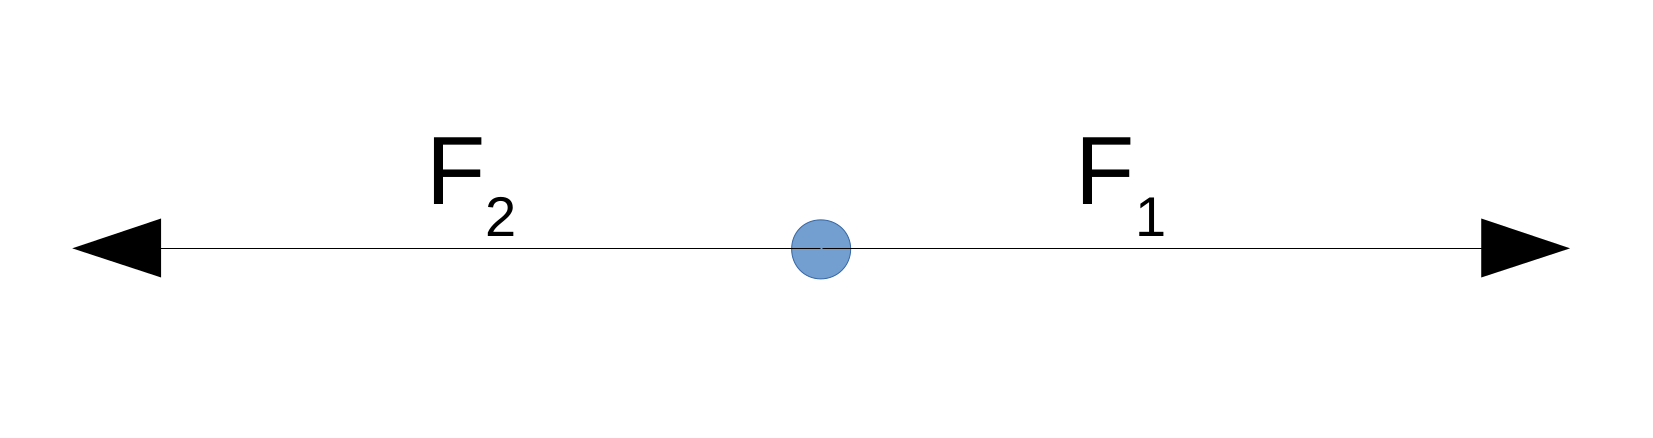
\includegraphics[width=0.7\textwidth]{kraefte_gleich}
	\caption{Gleich große, entgegengesetzte Kräfte: Es gibt keine resultierende Kraft.}
	\label{fig:kraefte_gleich}
\end{figure}

\noindent Bei zwei Kräften mit unterschiedlichem Betrag, die entgegengesetzt sind, müssen für den Betrag der Resultierenden die beiden Kräfte von einander abgezogen werden:

\begin{figure}[h!]
	\centering
	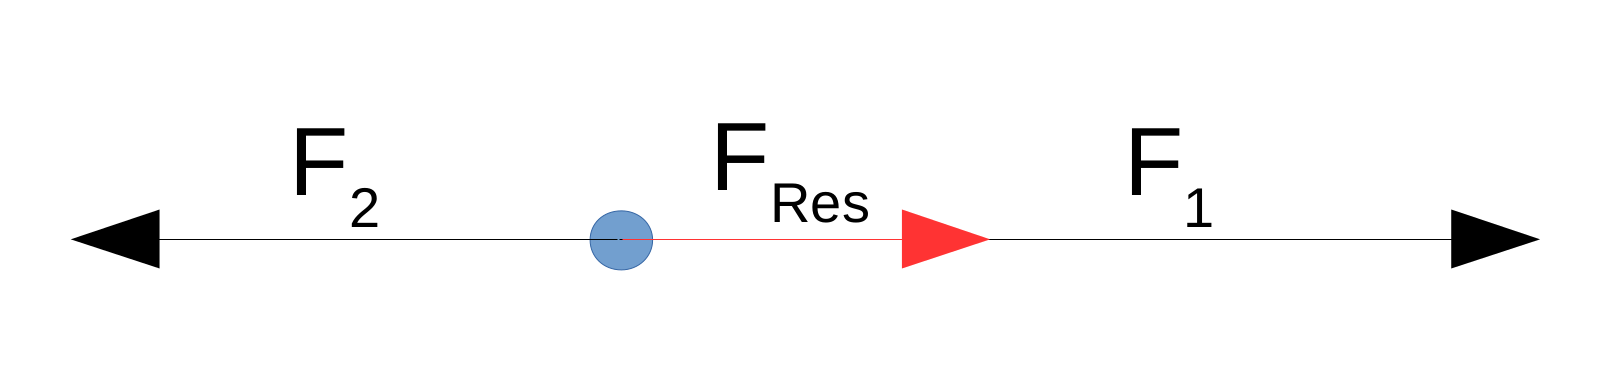
\includegraphics[width=0.7\textwidth]{kraefte_gleicherichtung}
	\caption{Entgegengesetzte Kräfte, mit unterschiedlichem Betrag.}
	\label{fig:kraefte_gleicherichtung}
\end{figure}

\subsubsection{Kräfte im rechten Winkel}

\noindent Die Pfeile von Kräften dürfen, z.B. zur erleichterten Herleitung von Gesetzen, verschoben werden, wenn ihre Länge und Richtung gewahrt werden. Dann wird kann der Fuß des einen Kraftpfeils an die Spitze des anderen Kraftpfeils angelegt und die Spitze zeigt dann die Spitze der Resultierenden an.

Dadurch ergibt sich aus dem Diagramm \ref{fig:kraefte_rechterwinkel} für zwei im rechten Winkel angreifende Kräfte mit dem Satz des Pythagoras:

\begin{align}
	F_{Res} = \sqrt{F_1^2 + F_2^2}
\end{align}

\begin{figure}[h!]
	\centering
	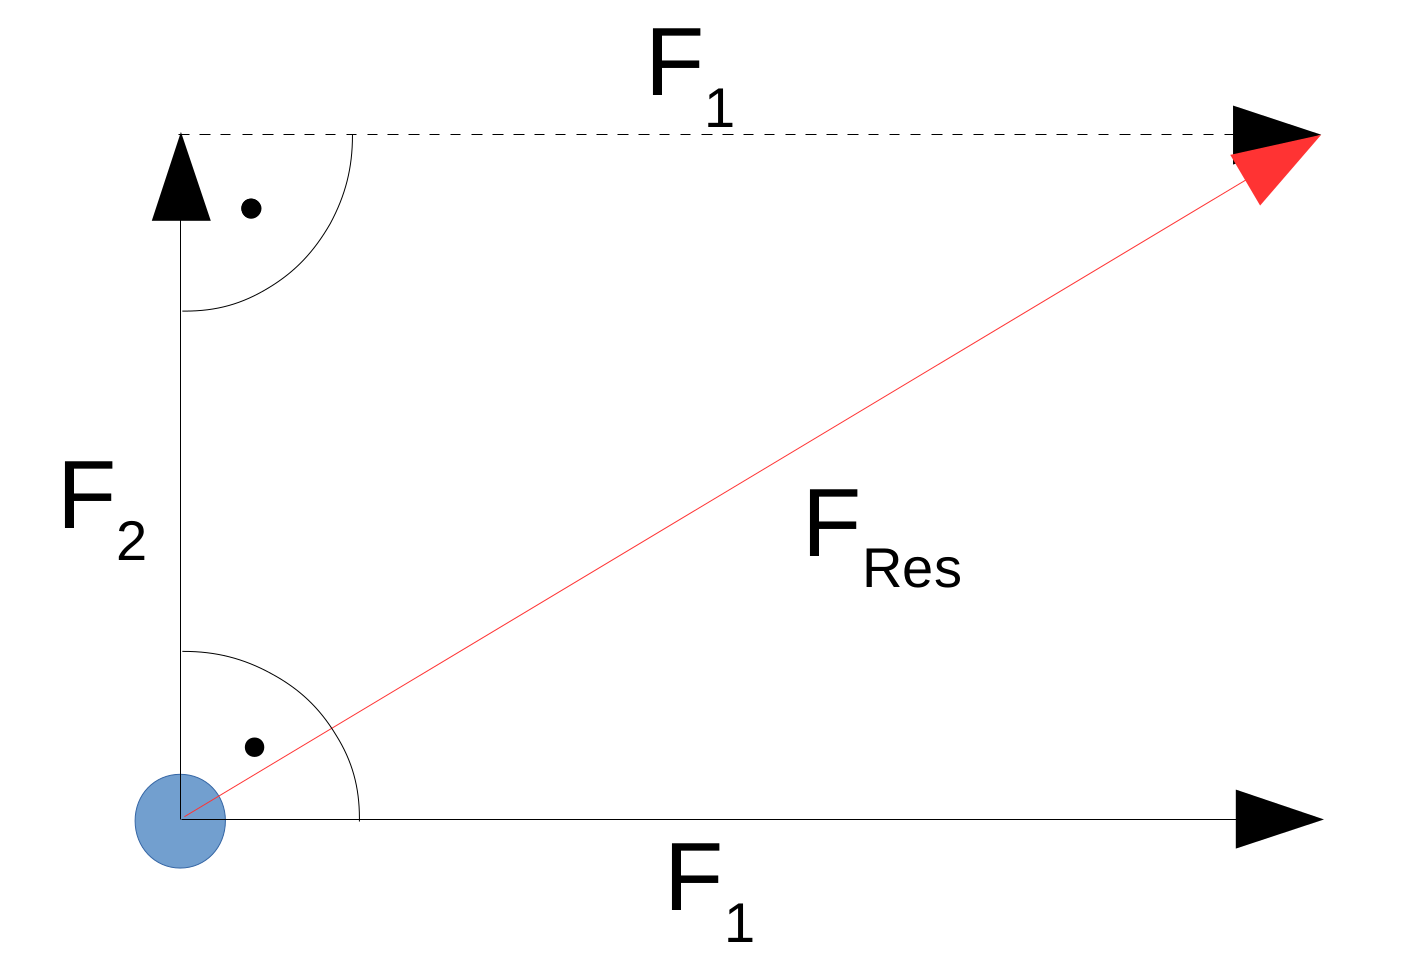
\includegraphics[width=0.7\textwidth]{kraefte_rechterwinkel}
	\caption{Kräfte im rechten Winkel}
	\label{fig:kraefte_rechterwinkel}
\end{figure}


\subsubsection{Kräfte im beliebigen Winkel}

\noindent Für einen beliebigen Winkel zwischen den Pfeilen muss mit dem Kosinussatz der Betrag der übrigen Seite $F_{Res}$ ermittelt werden, wie hier in Grafik \ref{fig:kraefte_beliebig}\endnote{Abbildungen \ref{fig:kraefte_beliebig}-\ref{fig:kraefte_gleich} \glqq Kräfteaddition\grqq{} von Till Blaha - Eigene Werke. Lizenziert unter Gemeinfrei}:

\begin{align}
	F_{Res} = \sqrt{F_1^2 + F_2^2 - 2F_1 F_2 \cdot \cos{\alpha '}}
\end{align}

\begin{figure}[H]
	\centering
	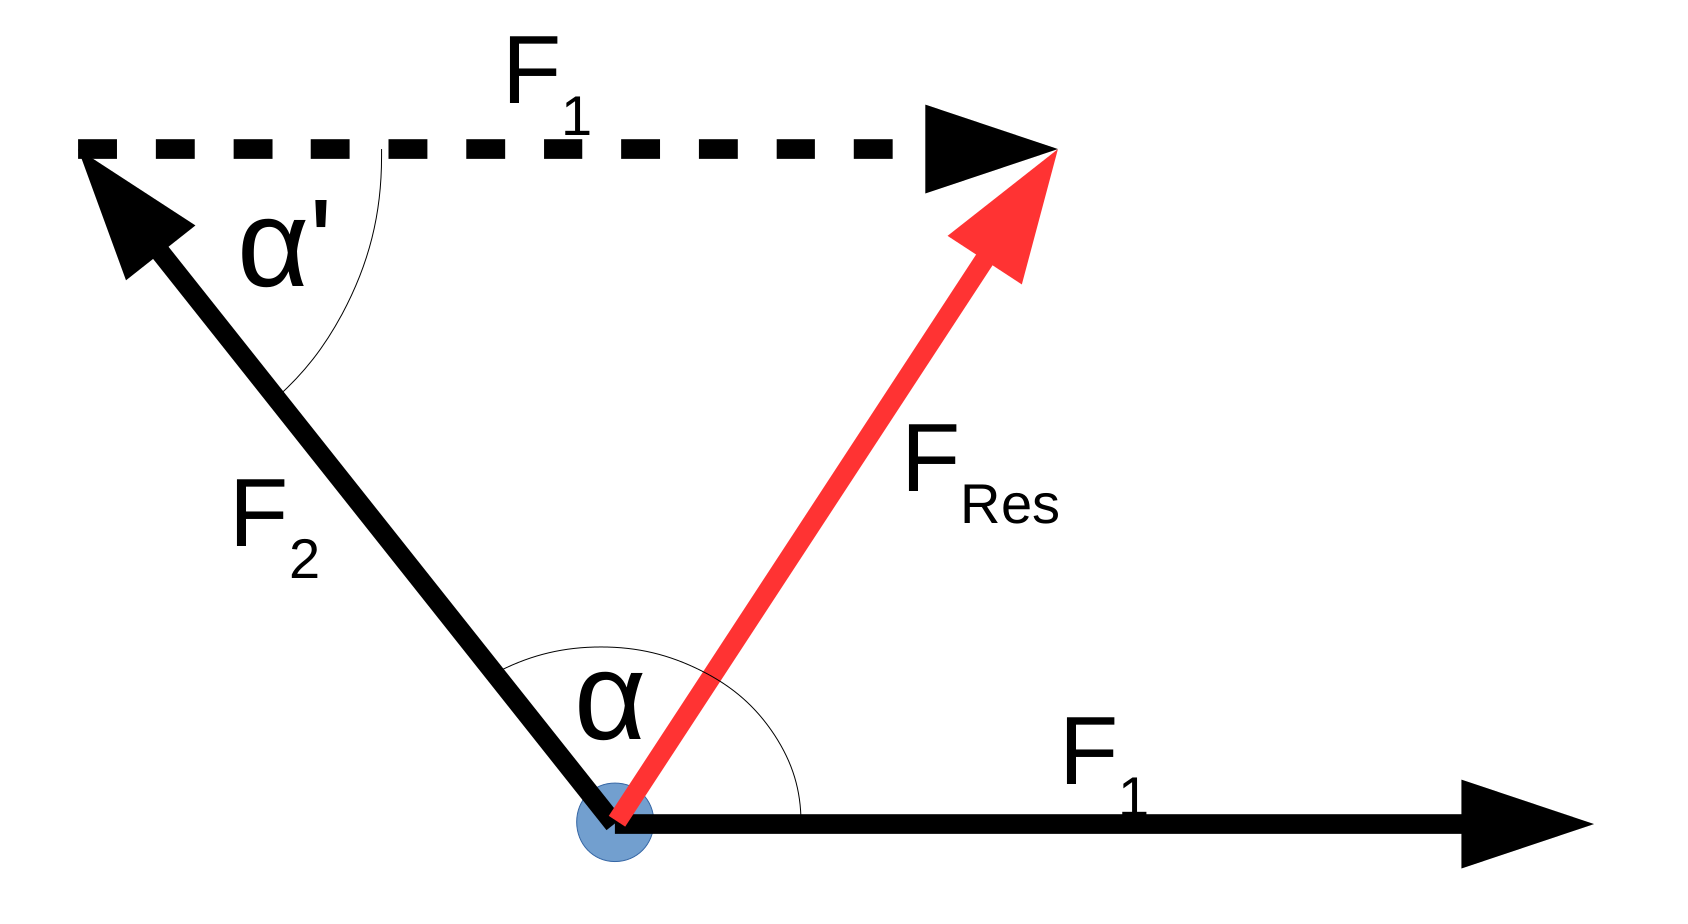
\includegraphics[width=0.7\textwidth]{kraefte_beliebig}
	\caption{Kräfte im beliebigen Winkel.}
	\label{fig:kraefte_beliebig}
\end{figure}


\subsection{Kräftesystem}

Aus dem dritten Newton'schen Axiom kann gefolgert werden, dass in einem abgeschlossenen Kräftesystem die Summe aller Kräfte $0$ sein muss, da jede Kraft eine gleich große und exakt entgegengesetzte Gegenkraft provoziert.

Dies ist wichtig für einige Herleitungen, z.B. am Federpendel (Siehe: \referenz{subsec:gesetze_federpendel}).


\subsection{Gewichtskraft} \label{subsec:Gewichtskraft}

Die Gewichtskraft $F_{G}$ ist die Kraft, die in der Mechanik besondere Bedeutung hat. Sie ist die Kraft, die ein Gravitationsfeld auf einen Körper auswirkt. Sie ist gemäß $F = m \cdot a$ abhängig von einer Beschleunigung, in diesem Fall der Gravitation (Schwerkraft) $g$, auf der Erde $\approx 9,81 \frac{m}{s^2}$, und von der Masse des Körpers:

\begin{align}
	F_{G} = m \cdot g
\end{align}

\noindent Die Einheit bleibt logischerweise das Newton.